\documentclass[14pt]{extreport}
\usepackage{gost}
\usepackage{hyperref}
\usepackage{makecell}
\usepackage{ragged2e}
\justifying

\begin{document}
\pagestyle{empty} 
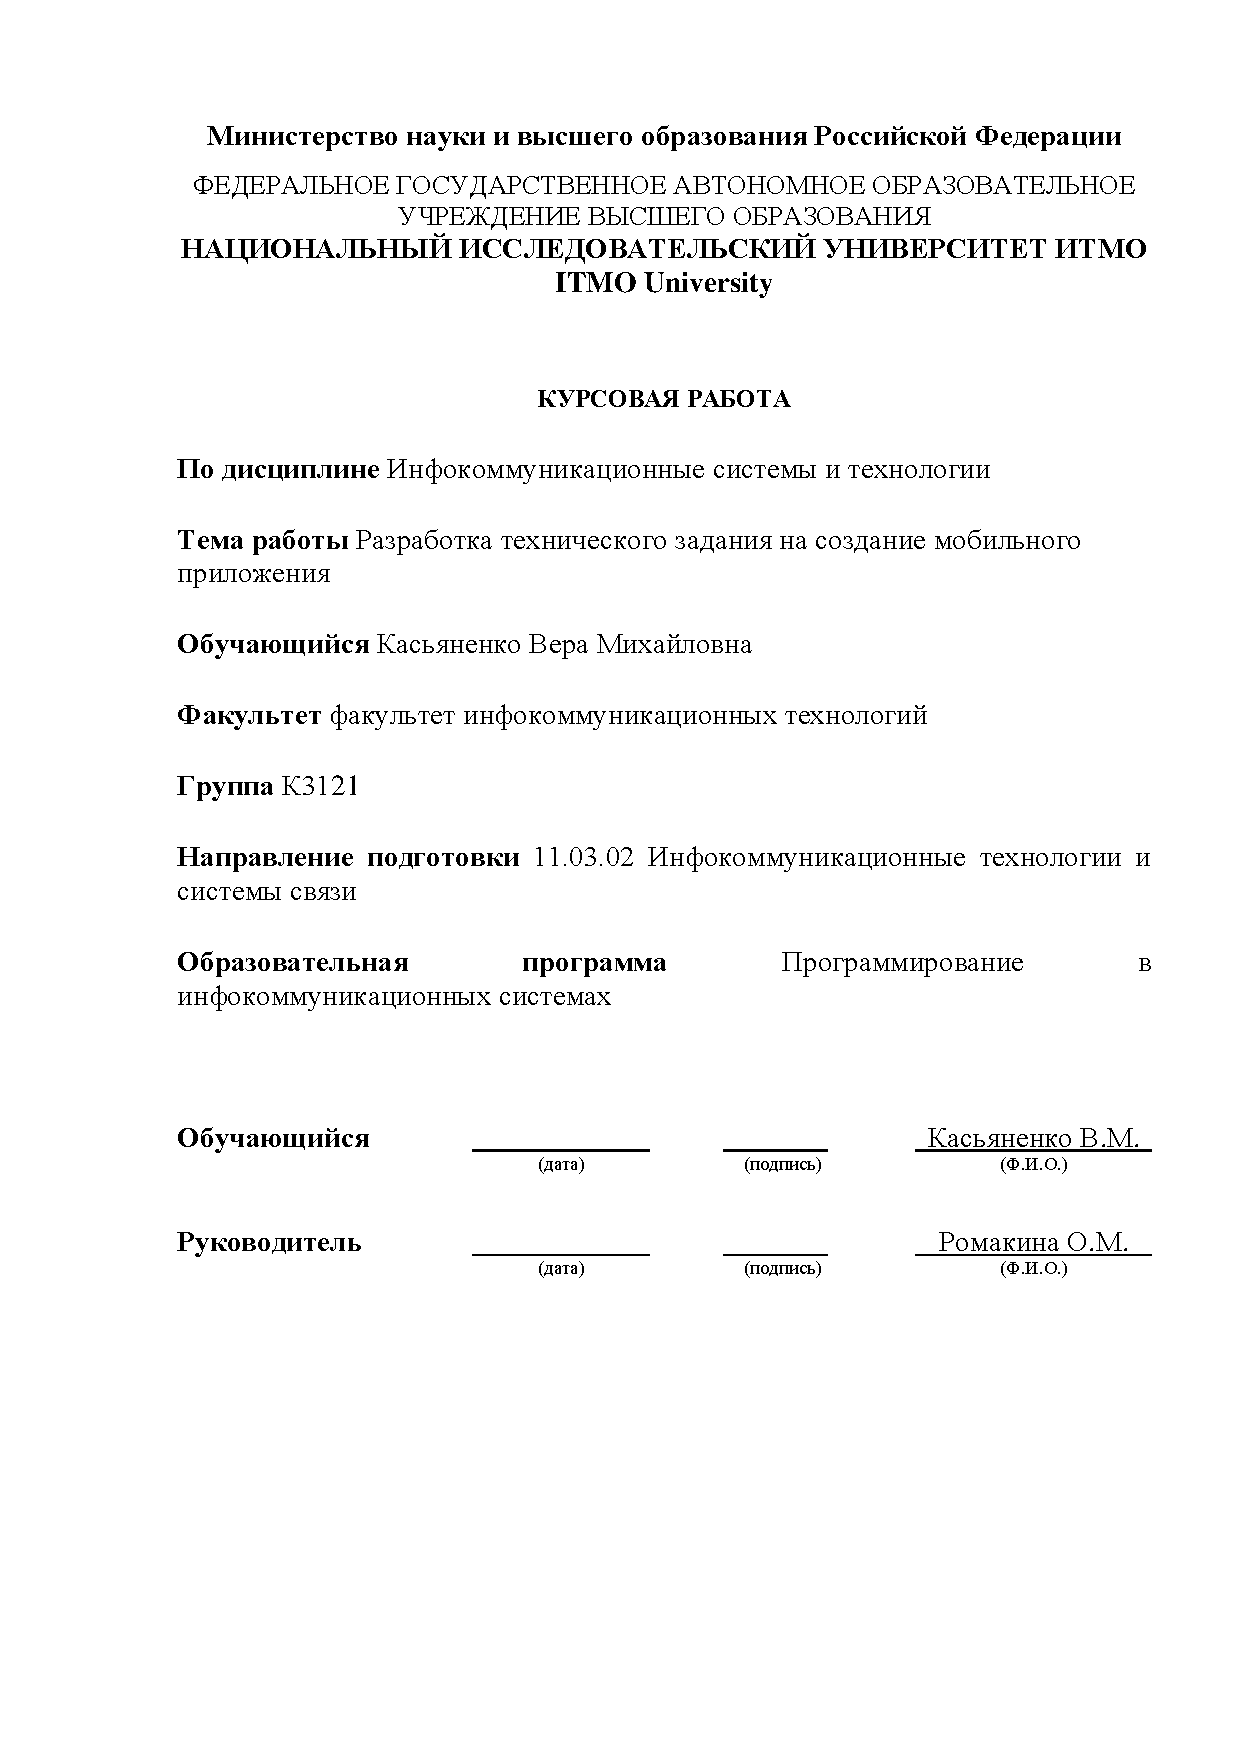
\includepdf[pages=-,pagecommand={}]{titulCourse.pdf}

\pagestyle{plain}

\newpage
\begin{center}
\begin{normalsize}
\textbf{АННОТАЦИЯ}
\end{normalsize}
\end{center}

Тема курсового проекта: Разработка технического задания на создание мобильного приложения

Выполнила - Касьяненко В.М.

Руководитель - Ромакина О.М.

Работа состоит из: введения, двух глав, заключения и списка используемых источников (8 наименований).

Во введении обоснована актуальность темы курсовой работы, цель и задачи.

В первой главе «Анализ предметной области» описаны предметная область и необходимые функции будущего приложения, подлежащие реализации, проведен обзор аналогов, а также представлены модели UML и диаграммы IDEF0, DFD, IDEF3 для будущего приложения.

Во второй главе «Создание технического задания на создание мобильное приложение» представлено разработанное техническое задание.

В заключении приведены основные выводы, полученные в результате написания курсовой работы.

Ключевые слова: мобильное приложение, тюнинг, оружие.

Работа состоит из 51 страницы, содержит 22 рисунка.

\newpage
\tableofcontents

\intro 

Актуальность темы исследования обусловлена тем, что огнестрельное оружие - это неотъемлемая часть современного мира. Для улучшения точности и удобства стрельбы профессиональные стрелки часто прибегают к модификации оружия при помощи установки на него различного тюнинга. 

В настоящее время существует множество видов различного тюнинга, однако стрелки, приходя в оружейный магазин не всегда могут оценить удобство и качество той или иной запчасти, так как нет достаточных сведений об ее использовании на практике. 

Мобильное приложение OptiTune поможет решить эти проблемы, так как пользователи смогут заранее просмотреть весь доступный тюнинг в большом каталоге, а также обменяться опытом использования этого тюнинга, что позволит быстрее и качественнее сделать свой выбор. Поэтому, действительно, есть смысл разработать техническое задание, которое поможет реализовать данное приложение, раскрыв все нюансы.

Целью курсовой работы является разработка технического задания на мобильное приложение OptiTune.

В связи с поставленной целью, необходимо решить следующие задачи:
\begin{itemize}
	\item описать необходимые функции приложения, подлежащих реализации;
	\item проанализировать и провести сравнение с аналогами, представленными на рынке;
	\item разработать модели UML, а также диаграммы IDEF0, DFD и IDEF3 для будущего приложения;
	\item создать техническое задание на создание мобильного приложения.
\end{itemize}

\chapter{Анализ предметной области}
\section{Описание предметной области и необходимых функций \\
будущего мобильного приложения, подлежащих реализации}

\subsection{Описание основных функций приложения}

Мобильное приложение OptiTune предназначено для использования профессиональными стрелками, охотниками и военными. Оно позволит подобрать тюнинг для гладкоствольного и нарезного оружия, улучшив там самым качество стрельбы на охоте, стрелковых соревнованиях и при выполнении различных военных заданий.

Используя приложение, пользователи смогут найти конкретное оружие, которое у них уже имеется или которое они только собираются приобрести, а также добавить его в избранное. Пользователи смогут посмотреть весь доступный тюнинг на их оружие и увидеть, как он будет выглядеть отдельно и на оружии, благодаря использованию 3D-моделей. Эту модель можно будет масштабировать и разглядывать с разных ракурсов, что позволит пользователю оценить насколько внешне подходит данная комплектация.

Для каждой запчасти будет доступна к просмотру и сравнению подробная характеристика, в которую входят такие параметры как высота, ширина, толщина, материал, из которого изготовлена запчасть, вес, примерная цена и другие характеристики, доступные для данной запчасти. По этим параметрам можно настроить сортировку и ускорить поиск. Таким образом, пользователи смогут правильнее оценить эти критерии и сделать выбор, который подходит именно им, а также добавить его в избранное.

Еще одной функцией приложения являются комментарии пользователей к запчастям. Пользователи смогут писать комментарии и прикреплять к ним фотографии и видеозаписи. Важно отметить, что функция написания будет доступна только зарегистрированным пользователям. Все комментарии будут проверяться модератором, чтобы избежать нежелательной информации.

В случае если у пользователя возникнут вопросы по техническим характеристикам или выбору, ему необходимо зарегистрироваться в приложении. Так, он сможет обратиться через специальное окно к онлайн-консультанту, который постарается ответить на все вопросы в ближайшее время.

Основной функционал, который будет представлен в приложении:
\begin{itemize}
	\item подбор тюнинга на основе конкретного оружия;
	\item просмотр тюнинга в 3D-варианте отдельно и на оружии;
	\item просмотр и сравнение характеристик запчастей;
	\item добавление в избранное понравившегося тюнинга;
	\item написание и просмотр комментариев пользователями;
	\item помощь онлайн-консультанта.
\end{itemize}

\subsection{Основные пользователи приложения}

Основными пользователями приложения являются люди, которые заинтересованы в тюнинге своего оружия. Им будут доступны такие функции как просмотр и подбор тюнинга, а также сравнение и добавление запчастей в избранное. Для зарегистрированных пользователей будет доступно написание комментариев и помощь онлайн-консультанта, в то время как для остальных пользователей будет доступен только просмотр оценок и комментариев этих пользователей.

Для того чтобы не допускать нежелательные комментарии и спам до обычных пользователей, необходим модератор, который будет отслеживать подобные комментарии.

Для помощи в каких-либо вопросах по характеристикам тюнинга и выбору нужен консультант, имеющий необходимые знания и отвечающий на эти вопросы.

Также важен менеджер, который будет обновлять информацию в приложении, например добавлять или удалять характеристики тюнинга.

\newpage
\section{Обзор аналогов, представленных на рынке}

При анализе зарубежного и российского рынка приложений не нашлось аналогов. Лишь среди сайтов можно было отыскать что-то похожее.

Интернет-магазин товаров для тюнинга оружия и аксессуаров Custom Guns \cite{bib1}. На данном сайте можно найти и купить запчасти. На сайте есть иллюстрации к каждой запчасти, цена и подробные характеристики. Так же как и у моего приложения здесь есть система оценивания и онлайн-консультанта. Однако на сайте нельзя сравнивать и добавлять в избранное запчасти, также нельзя посмотреть как тюнинг будет выглядеть на оружии, зато настроен интернет-магазин.

В двух других интернет-магазинах, QUARTA \cite{bib2} и Guns Parts \cite{bib3}, так же присутствовали иллюстрации к тюнингу, сортировка, отзывы о товаре и онлайн-консультант. В отличие от первого сайта, здесь пользователь может зайти в личный кабинет и добавить товары в избранное. Однако все еще нельзя посмотреть внешний вид оружия с тюнингом. 

Во всех трех системах целевая аудитория совпадает с целевой аудиторией приложения. Важно отметить, что довольно сложно сделать 3D-модели для всех запчастей, поэтому большая часть систем не воплощает эту идею. 

\newpage
\section{Обоснование необходимости разработки}

Проанализировав рынок приложений в предыдущем разделе, не сложно заметить, что конкуренции в этой области нет, а также это уникальное приложение, которое может заинтересовать профессиональных стрелков своим функционалом, позволяющим ускорить процесс поиска и выбора необходимого тюнинга. Поэтому, действительно, есть смысл реализовать данное приложение.

\newpage
\section{Разработка диаграмм прецедентов и активности для \\ типовых сценариев работы приложения}

Для лучшего понимания функционирования системы были созданы диаграммы прецедентов и активности на языке UML, которые значительно упростят понимание логики приложения, а также помогут при создании технического задания.

\subsection{Диаграммы прецедентов}

В данном подразделе представлены диаграммы прецедентов на языке UML, описывающие функциональное назначение мобильного приложения. Для более удобного восприятия они были разделены на диаграммы для незарегистированных (рисунок \ref{fig1}) и зарегистрированных пользователей (рисунок \ref{fig2}), а также для членов административной группы (рисунок \ref{fig3}). Выполнено с помощью \cite{bib4}.

\begin{figure}[H]
\centerline{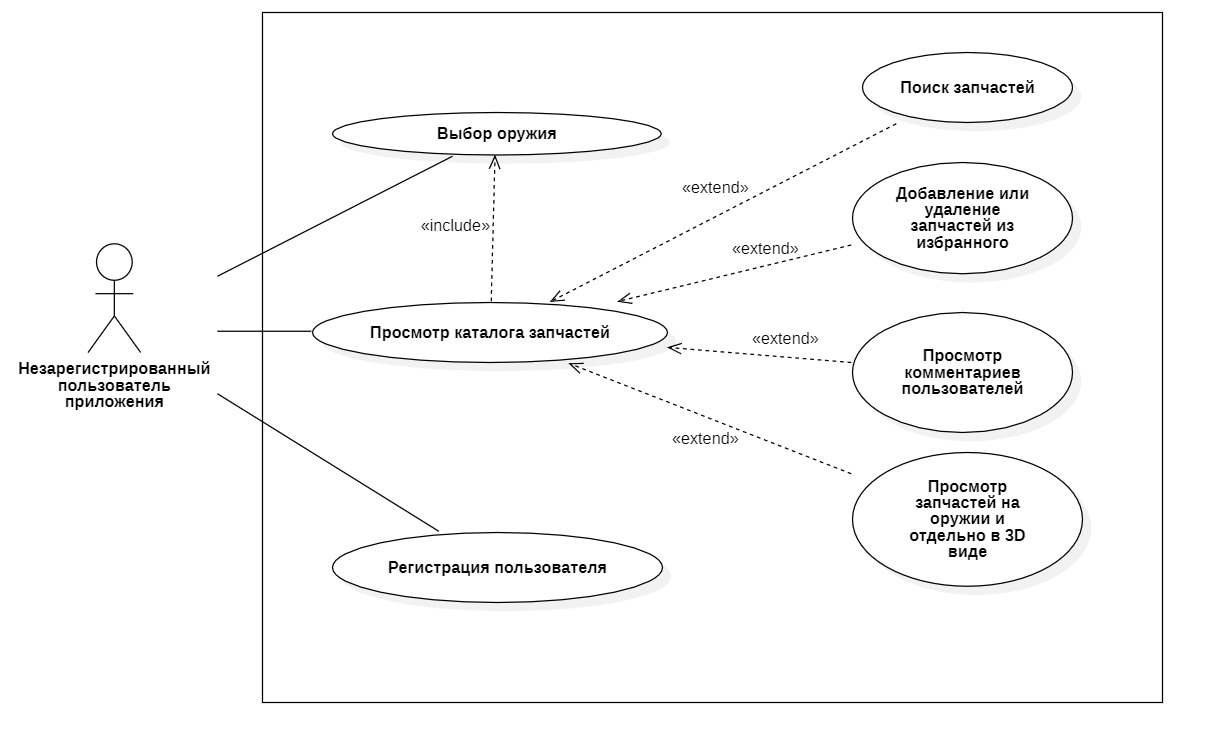
\includegraphics[width=1\linewidth]{nereg}}
\caption{Диаграмма прецедентов для пользователей без регистрации}
\label{fig1}
\end{figure}

\begin{figure}[H]
\centerline{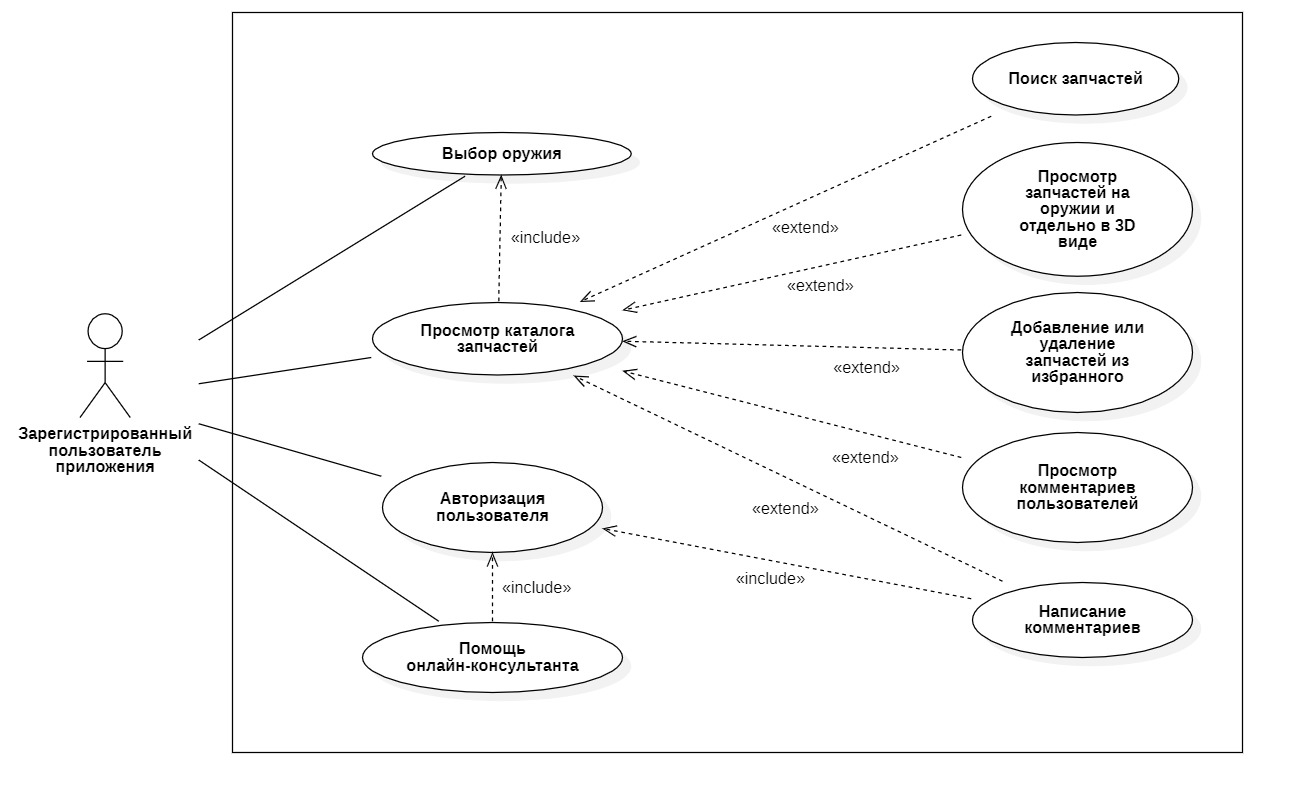
\includegraphics[width=1\linewidth]{reg}}
\caption{Диаграмма прецедентов для пользователей c регистрацией}
\label{fig2}
\end{figure}

\begin{figure}[H]
\centerline{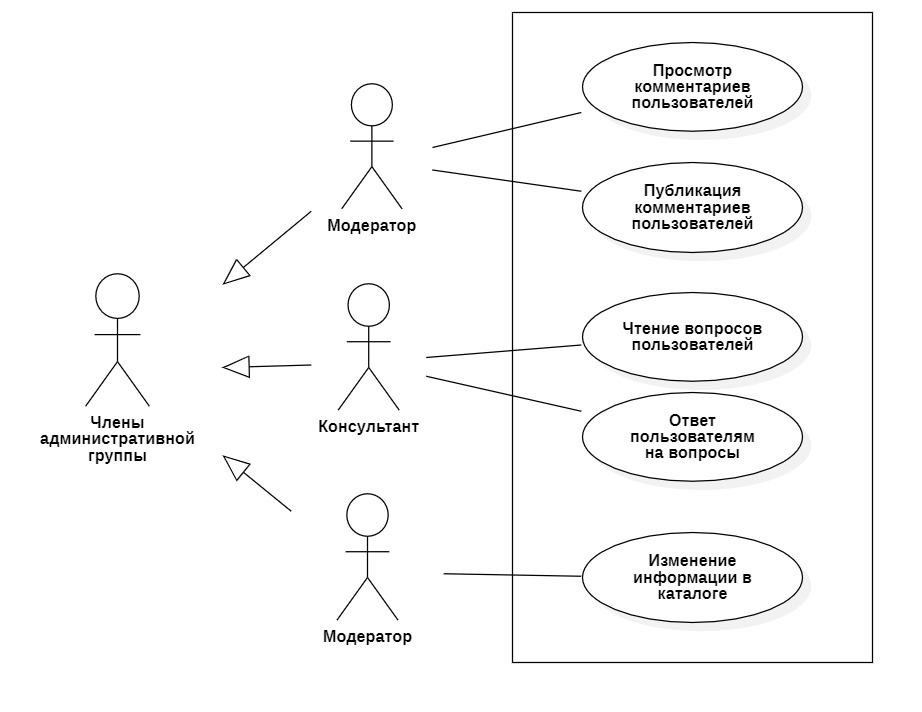
\includegraphics[width=0.7\linewidth]{adm}}
\caption{Диаграмма прецедентов для членов административной группы}
\label{fig3}
\end{figure}

\newpage
\subsection{Диаграммы активности для ключевых прецедентов}

В данном подразделе представлены диаграммы активности, описывающие процесс выполнения действий при работе приложения, для следующих прецедентов: авторизация пользователей (рисунок \ref{fig4}), использование каталога (рисунок \ref{fig5}), модерация комментариев (рисунок \ref{fig6}), помощь онлайн-консультанта (рисунок \ref{fig7}) и обновление менеджером информации в приложении (рисунок \ref{fig8}). Выполнено с помощью \cite{bib4}.

\begin{figure}[H]
\centerline{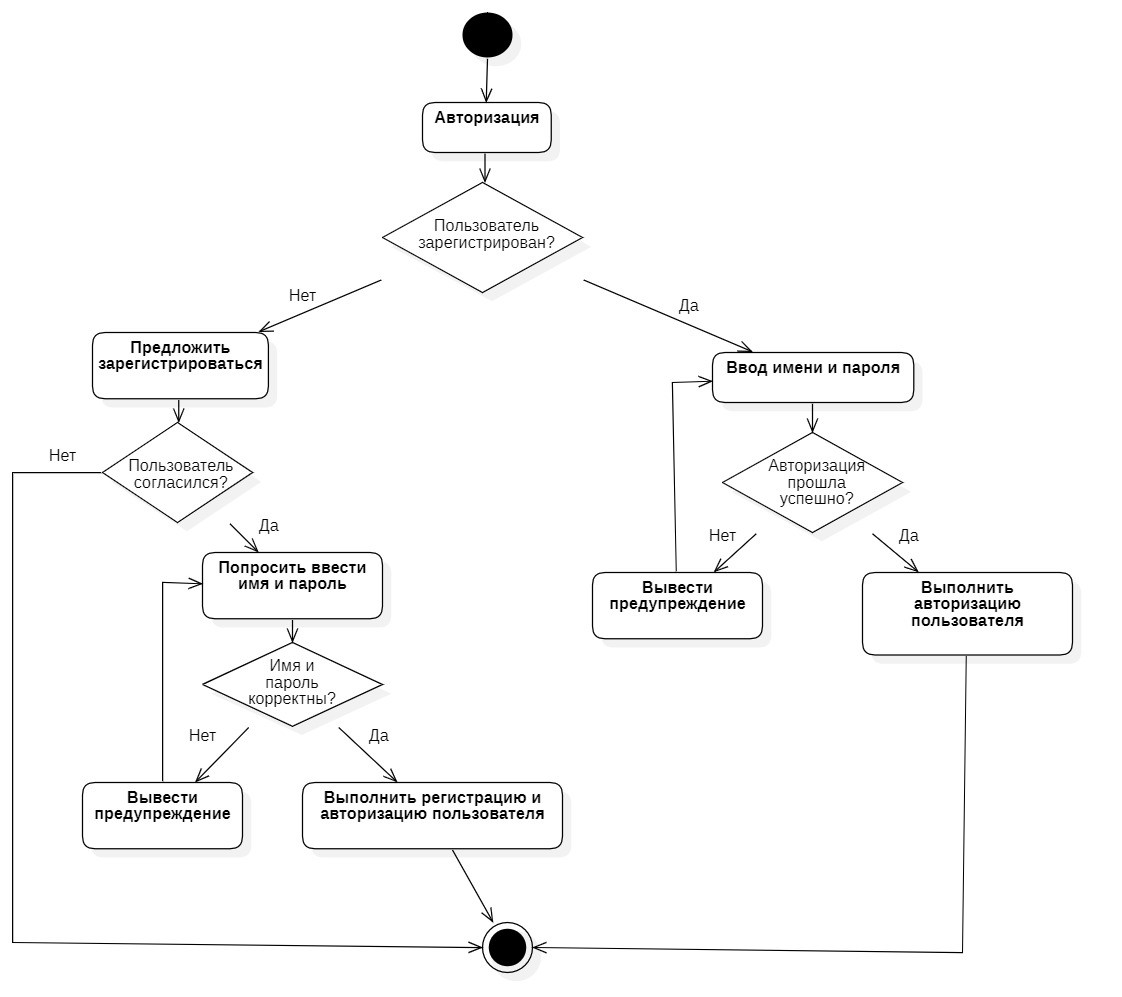
\includegraphics[width=1\linewidth]{act_avto}}
\caption{Диаграмма активности авторизации пользователей}
\label{fig4}
\end{figure}

\begin{figure}[H]
\centerline{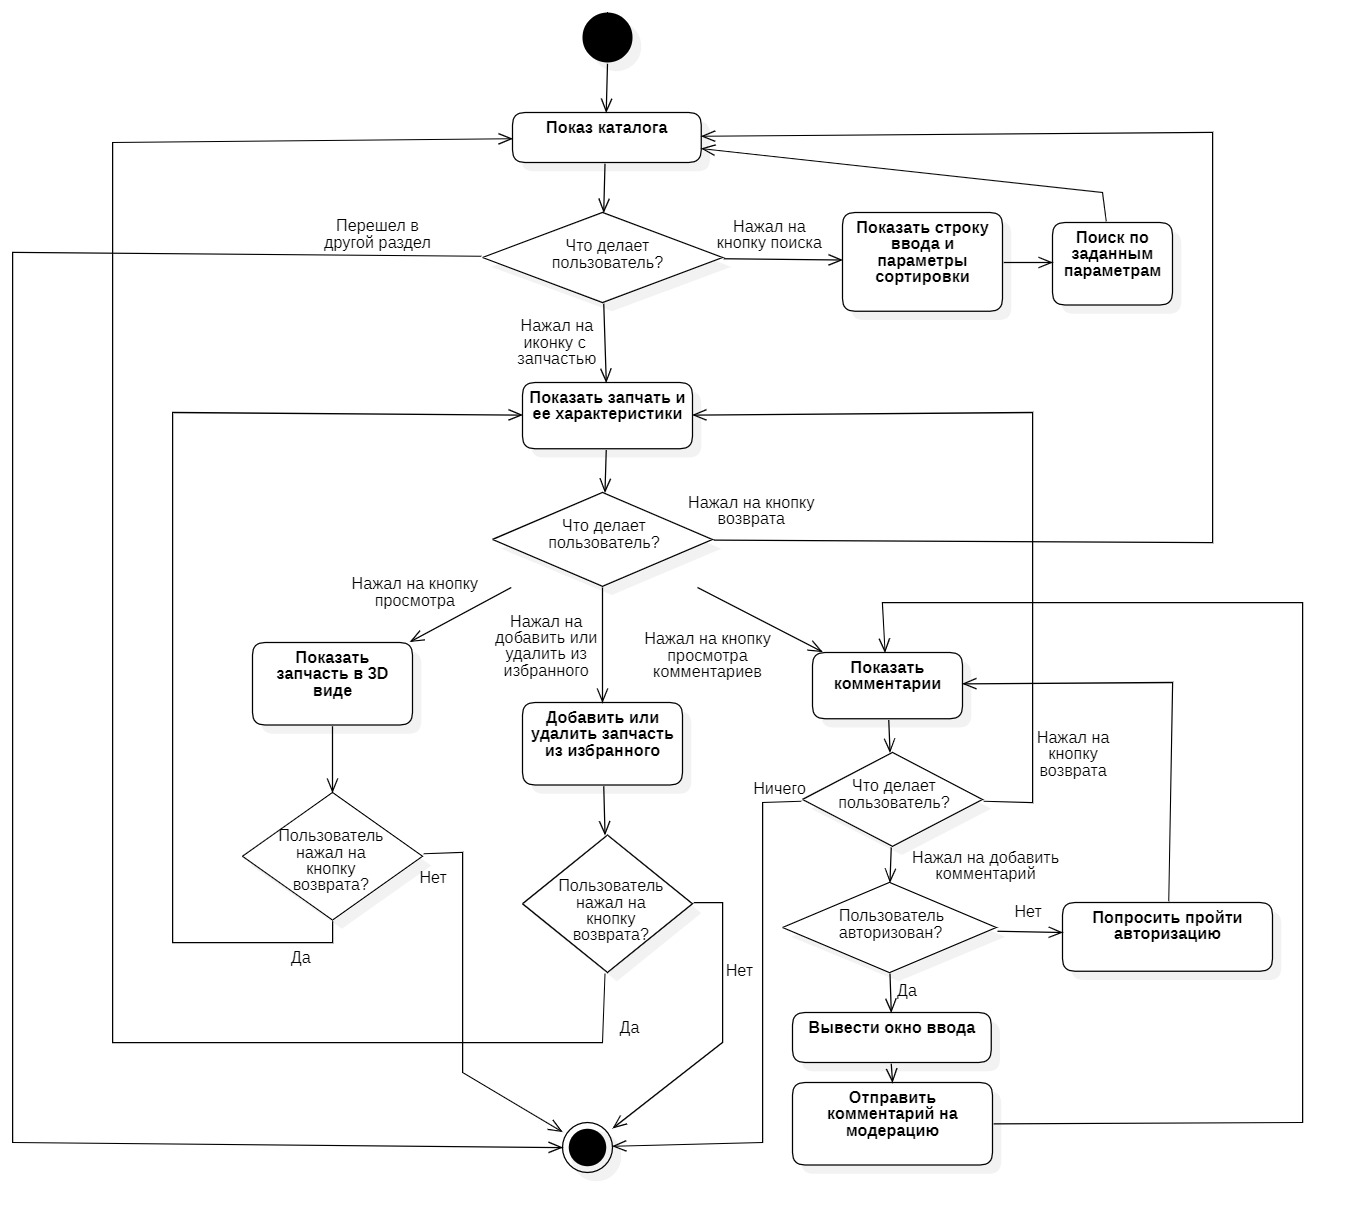
\includegraphics[width=1.05\linewidth]{act_pols}}
\caption{Диаграмма активности использования каталога пользователем}
\label{fig5}
\end{figure}

\begin{figure}[H]
\centerline{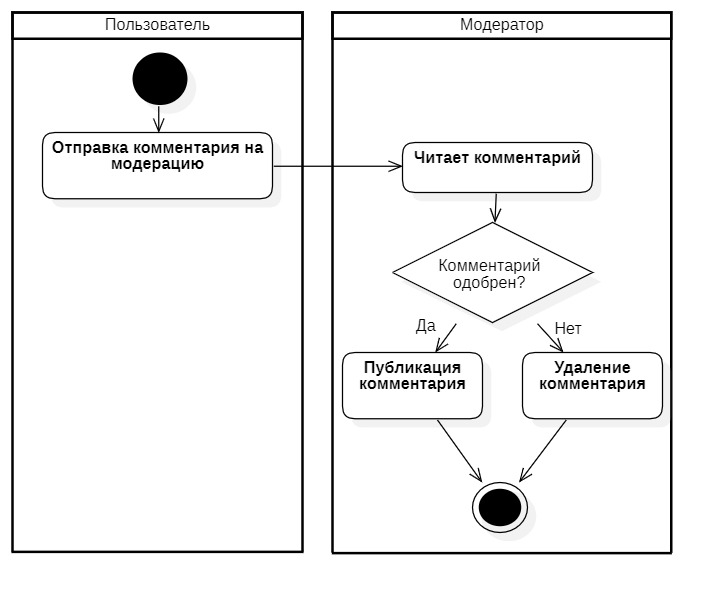
\includegraphics[width=0.6\linewidth]{act_kom}}
\caption{Диаграмма активности отправки комментария на модерацию}
\label{fig6}
\end{figure}

\begin{figure}[H]
\centerline{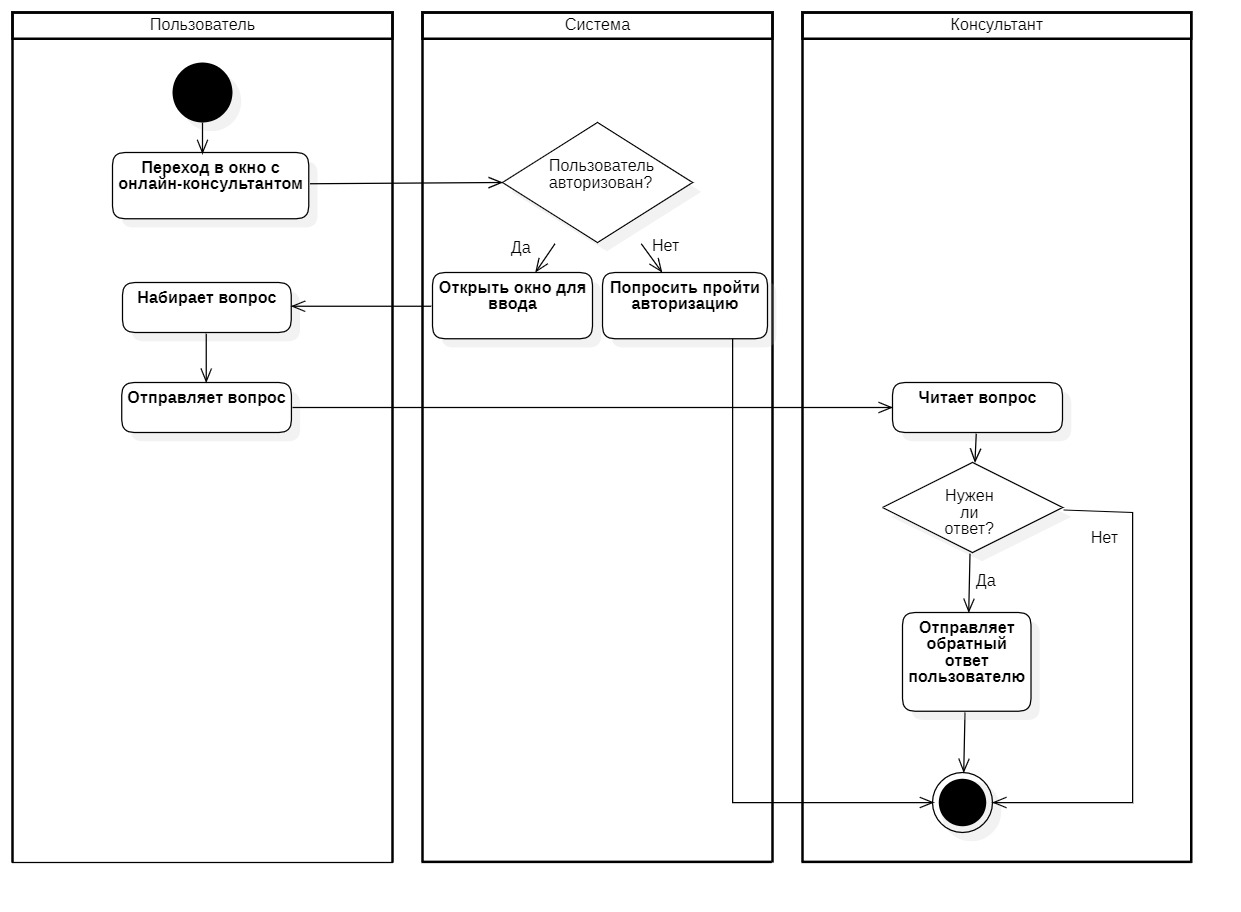
\includegraphics[width=0.9\linewidth]{act_kons}}
\caption{Диаграмма активности обращения к онлайн-консультанту}
\label{fig7}
\end{figure}

\begin{figure}[H]
\centerline{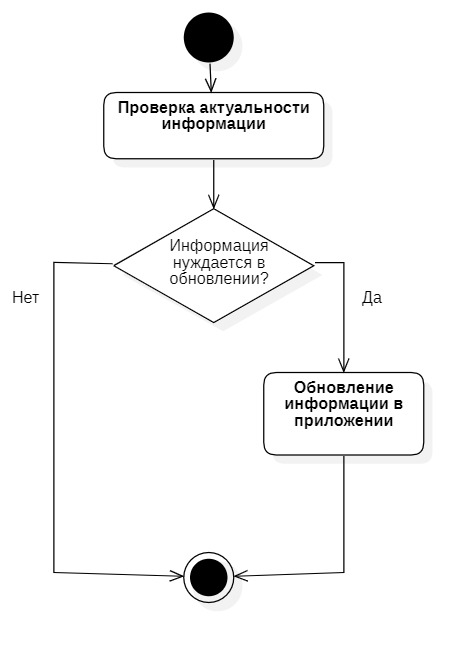
\includegraphics[width=0.5\linewidth]{act_men}}
\caption{Диаграмма активности обновления менеджером информации}
\label{fig8}
\end{figure}


\newpage
\section{Разработка диаграмм IDEF0, DFD, IDEF3 для будущего
приложения}

В данном разделе представлены диаграммы IDEF0, DFD, IDEF3, которые раскроют работу мобильного приложения, а также помогут при создании технического задания.

\subsection{Функциональные модели в стандарте IDEF0}

В данном подразделе представлены функциональные модели в стандарте IDEF0 с точки зрения пользователя приложения OptiTune, которые описывают функционирование системы при подборе необходимого тюнинга. Модели представлены в виде контекстной диаграммы (рисунок \ref{fig9}) и декомпозиции этой диаграммы  (рисунок \ref{fig10}). Также для декомпозиции контекстной диаграммы представлены декомпозиции блоков "Определение уровня доступа в систему"\ (рисунок \ref{fig11}) и "Обработка запроса пользователя"\ (рисунок \ref{fig12}). Более того, для блока "Определение уровня доступа в систему"\ представлена декомпозиции блока "Авторизация"\ (рисунок \ref{fig13}). Выполнено с помощью \cite{bib5}.

\begin{landscape}
\begin{figure}[H]
\centerline{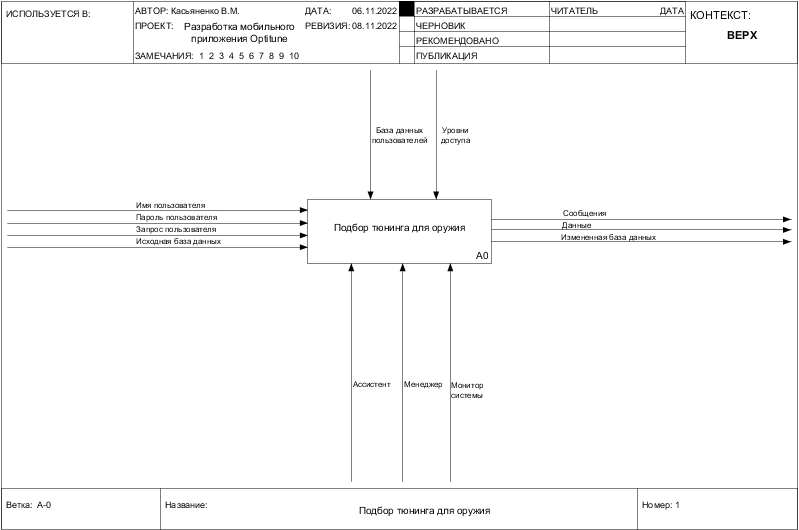
\includegraphics[width=0.9\linewidth]{01_A-0}}
\caption{Контекстная диаграмма}
\label{fig9}
\end{figure}

\begin{figure}[H]
\centerline{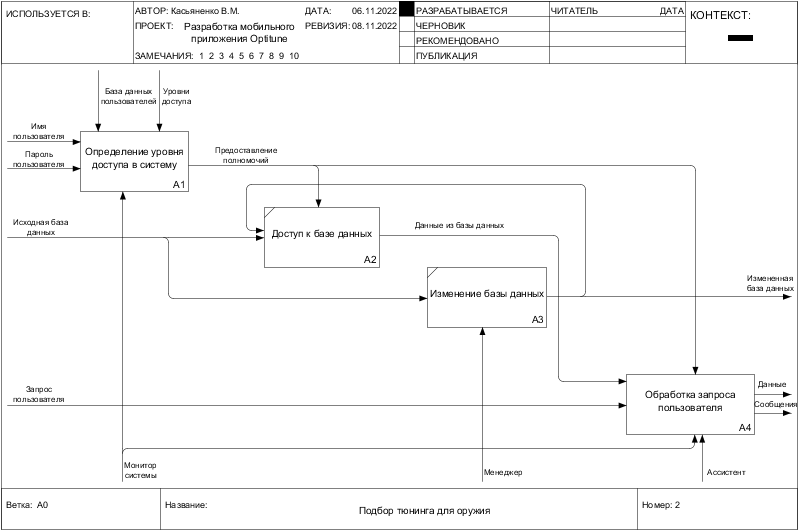
\includegraphics[width=0.9\linewidth]{02_A0}}
\caption{Декомпозиция контекстной диаграммы}
\label{fig10}
\end{figure}

\begin{figure}[H]
\centerline{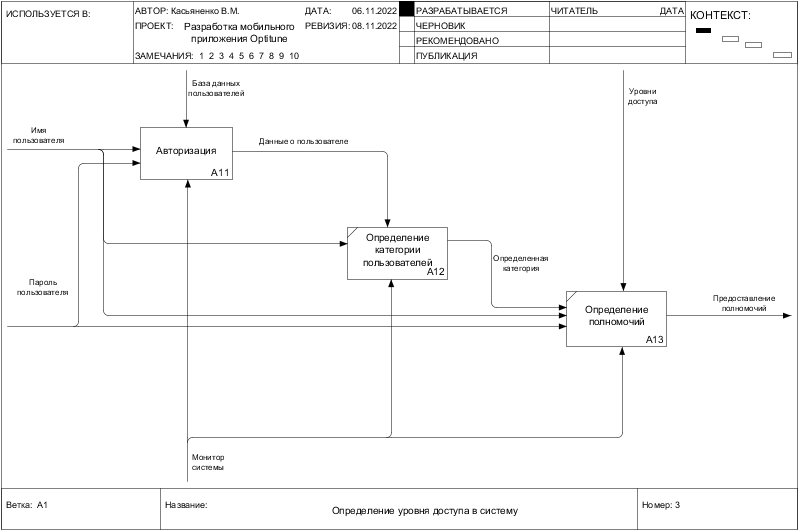
\includegraphics[width=0.9\linewidth]{03_A1}}
\caption{Декомпозиция блока "Определение уровня доступа в систему"}
\label{fig11}
\end{figure}

\begin{figure}[H]
\centerline{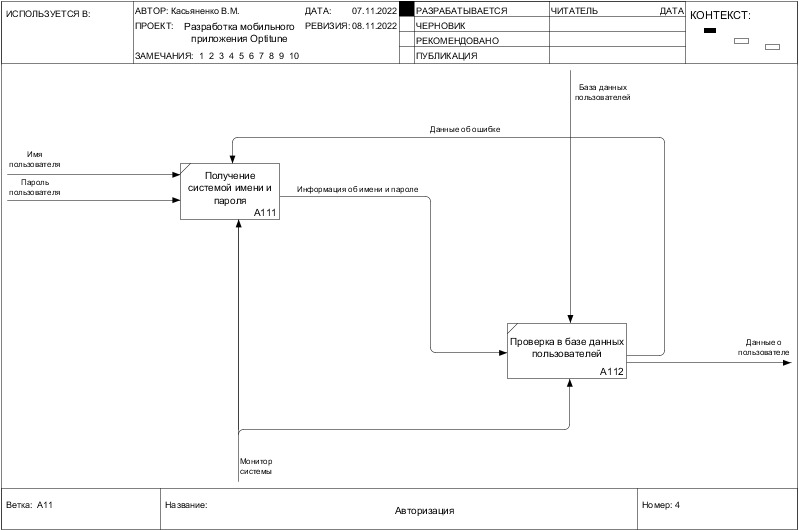
\includegraphics[width=0.9\linewidth]{04_A11}}
\caption{Декомпозиция блока "Авторизация"}
\label{fig12}
\end{figure}

\begin{figure}[H]
\centerline{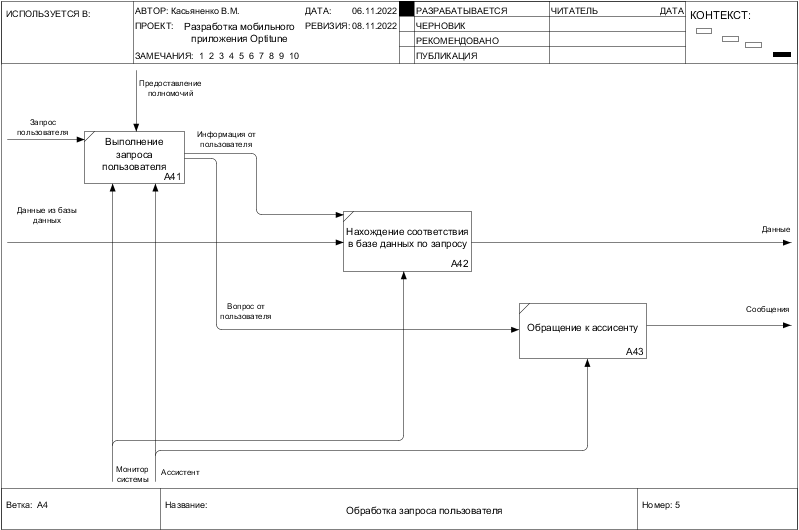
\includegraphics[width=0.9\linewidth]{05_A4}}
\caption{Декомпозиция блока "Обработка запроса пользователя"}
\label{fig13}
\end{figure}
\end{landscape}

\subsection{Диаграммы в стандарте DFD}

В данном подразделе представлены в стандарте диаграммы DFD, описывающие функции обработки информации. Они представлены как дополнение к диаграмме в стандарте IDEF0. В диаграмму в стандарте IDEF0 входит контекстная диаграмма  (рисунок \ref{fig14}) и декомпозиция этой диаграммы  (рисунок \ref{fig15}). Для этой декомпозиции контекстной диаграммы представлены  декомпозиции блоков "Определение уровня доступа в систему"\ (рисунок \ref{fig16}) и "Обработка запроса пользователя"\ (рисунок \ref{fig17}) в формате DFD. Выполнено с помощью \cite{bib5}.

\begin{landscape}
\begin{figure}[H]
\centerline{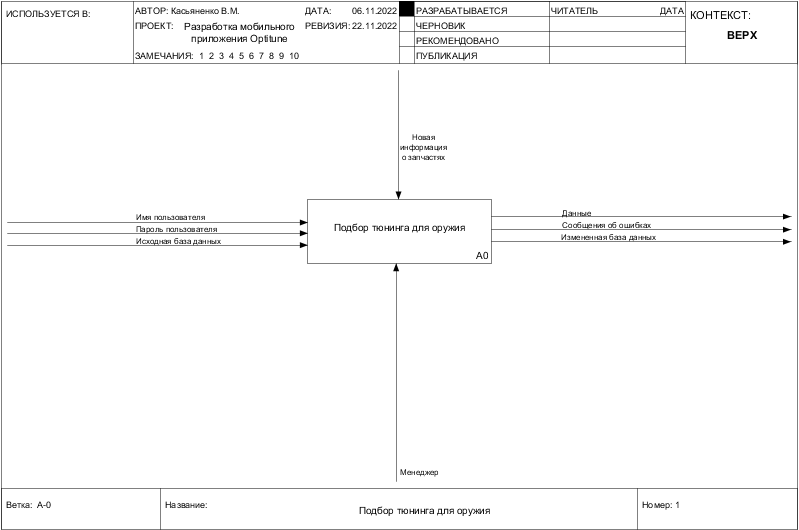
\includegraphics[width=0.9\linewidth]{dfd01_A-0}}
\caption{Контекстная диаграмма в стандарте IDEF0}
\label{fig14}
\end{figure}

\begin{figure}[H]
\centerline{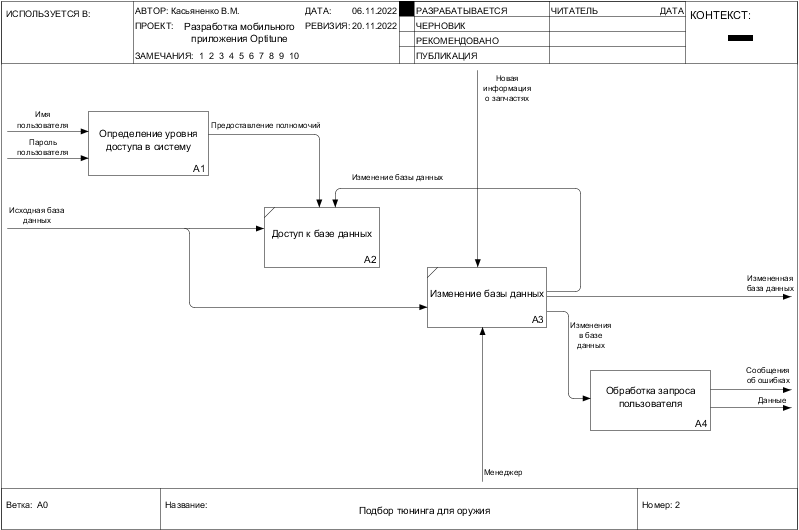
\includegraphics[width=0.9\linewidth]{dfd02_A0}}
\caption{Декомпозиция контекстной диаграммы в стандарте IDEF0}
\label{fig15}
\end{figure}

\begin{figure}[H]
\centerline{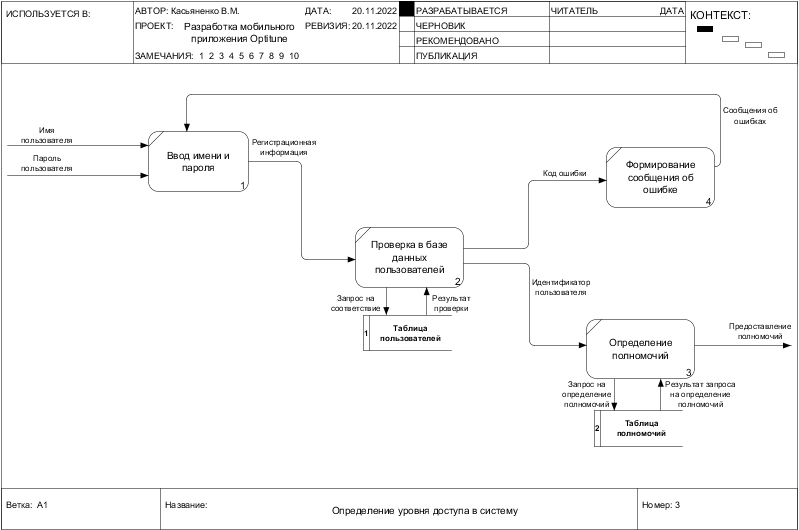
\includegraphics[width=0.9\linewidth]{dfd03_A1}}
\caption{Декомпозиция блока "Определение уровня доступа в систему"\ в стандарте DFD}
\label{fig16}
\end{figure}

\begin{figure}[H]
\centerline{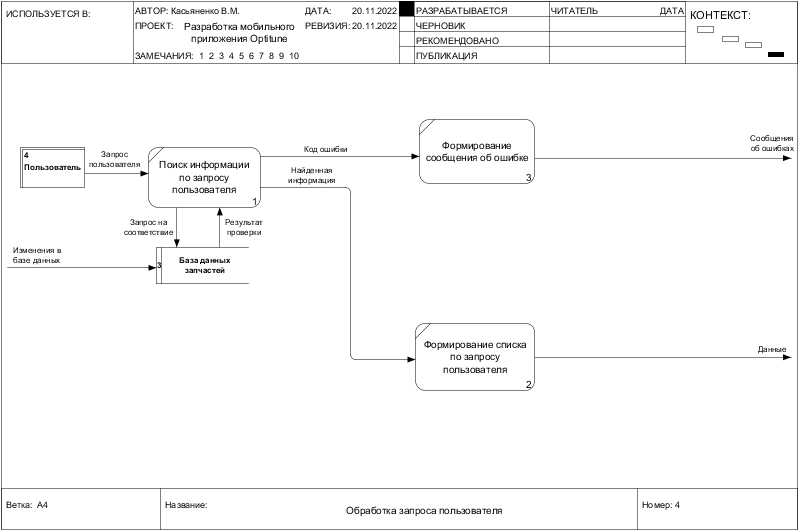
\includegraphics[width=0.9\linewidth]{dfd04_A4}}
\caption{Декомпозиция блока "Обработка запроса пользователя"\ в стандарте DFD}
\label{fig17}
\end{figure}
\end{landscape}

\subsection{Модель в стандарте IDEF3}

В данном подразделе представлена модель в стандарте IDEF3, описывающая информационные потоки, а также взаимоотношения между процессами обработки информации и объектов, являющихся частью этих процессов. Модель представлена в виде контекстной диаграммы  (рисунок \ref{fig18}) и декомпозиции этой диаграммы  (рисунок \ref{fig19}). Также для декомпозиции контекстной диаграммы представлены декомпозиции блоков "Определение уровня доступа в систему"\ (рисунок \ref{fig20}) и "Обработка запроса пользователя"\ (рисунок \ref{fig21}). Выполнено с помощью \cite{bib6}.

\begin{landscape}
\begin{figure}[H]
\centerline{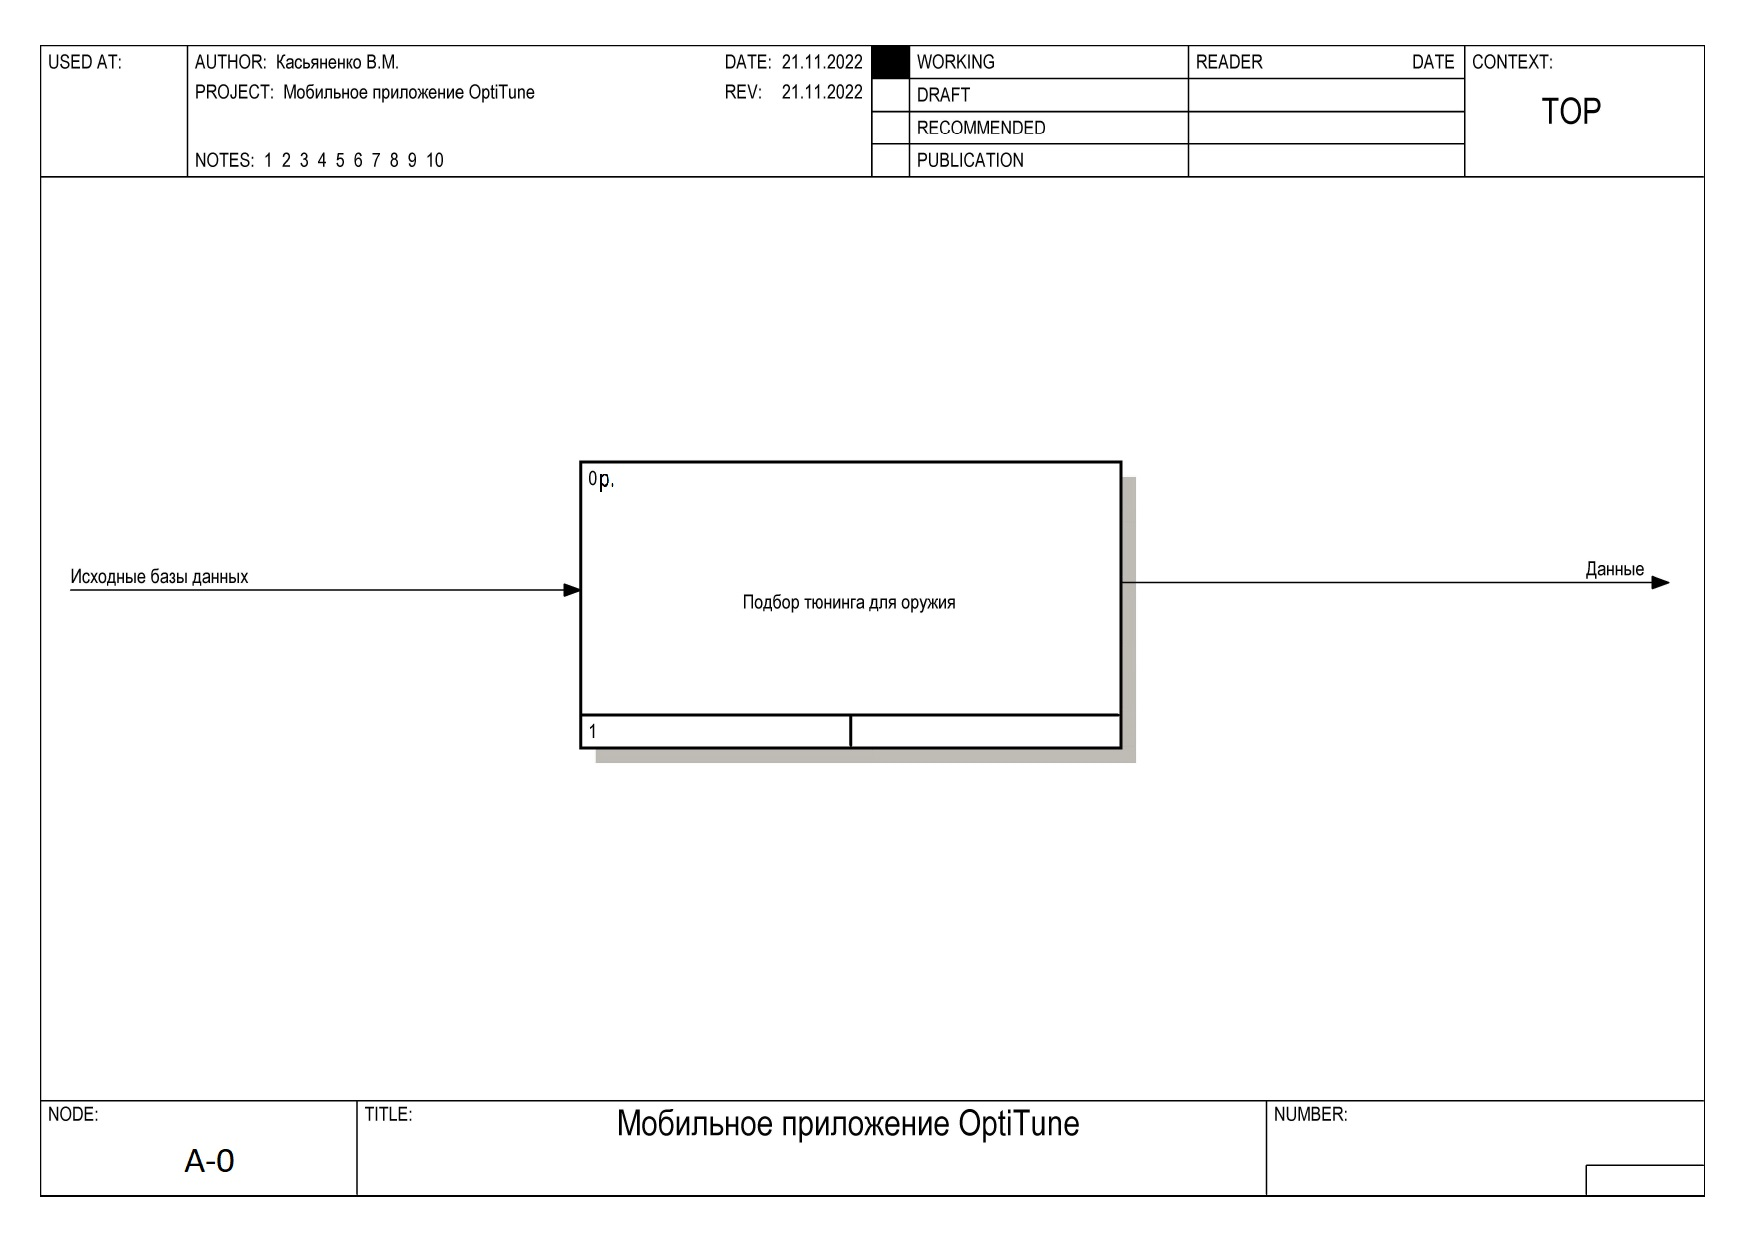
\includegraphics[width=0.9\linewidth]{idef30}}
\caption{Контекстная диаграмма в стандарте IDEF3}
\label{fig18}
\end{figure}

\begin{figure}[H]
\centerline{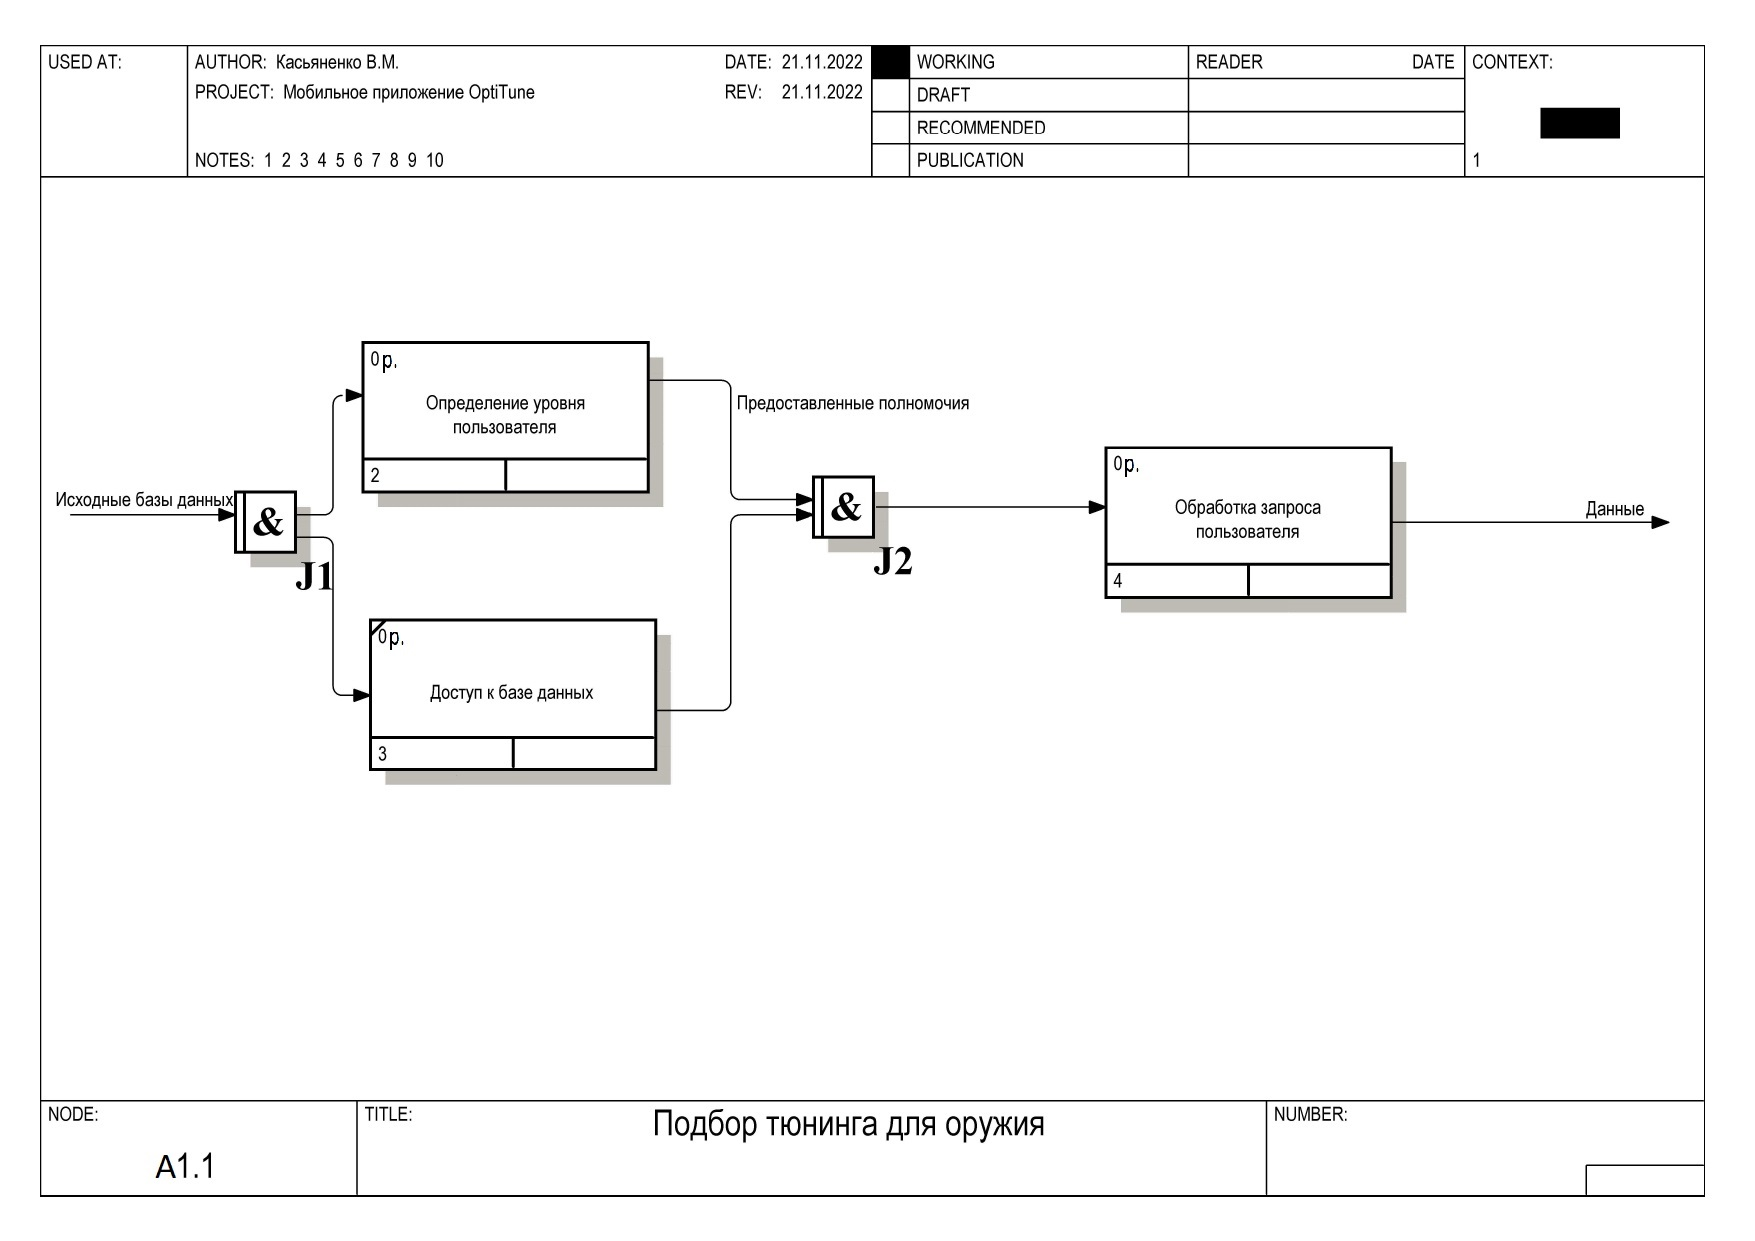
\includegraphics[width=0.9\linewidth]{idef31}}
\caption{Декомпозиция контекстной диаграммы в стандарте IDEF3}
\label{fig19}
\end{figure}

\begin{figure}[H]
\centerline{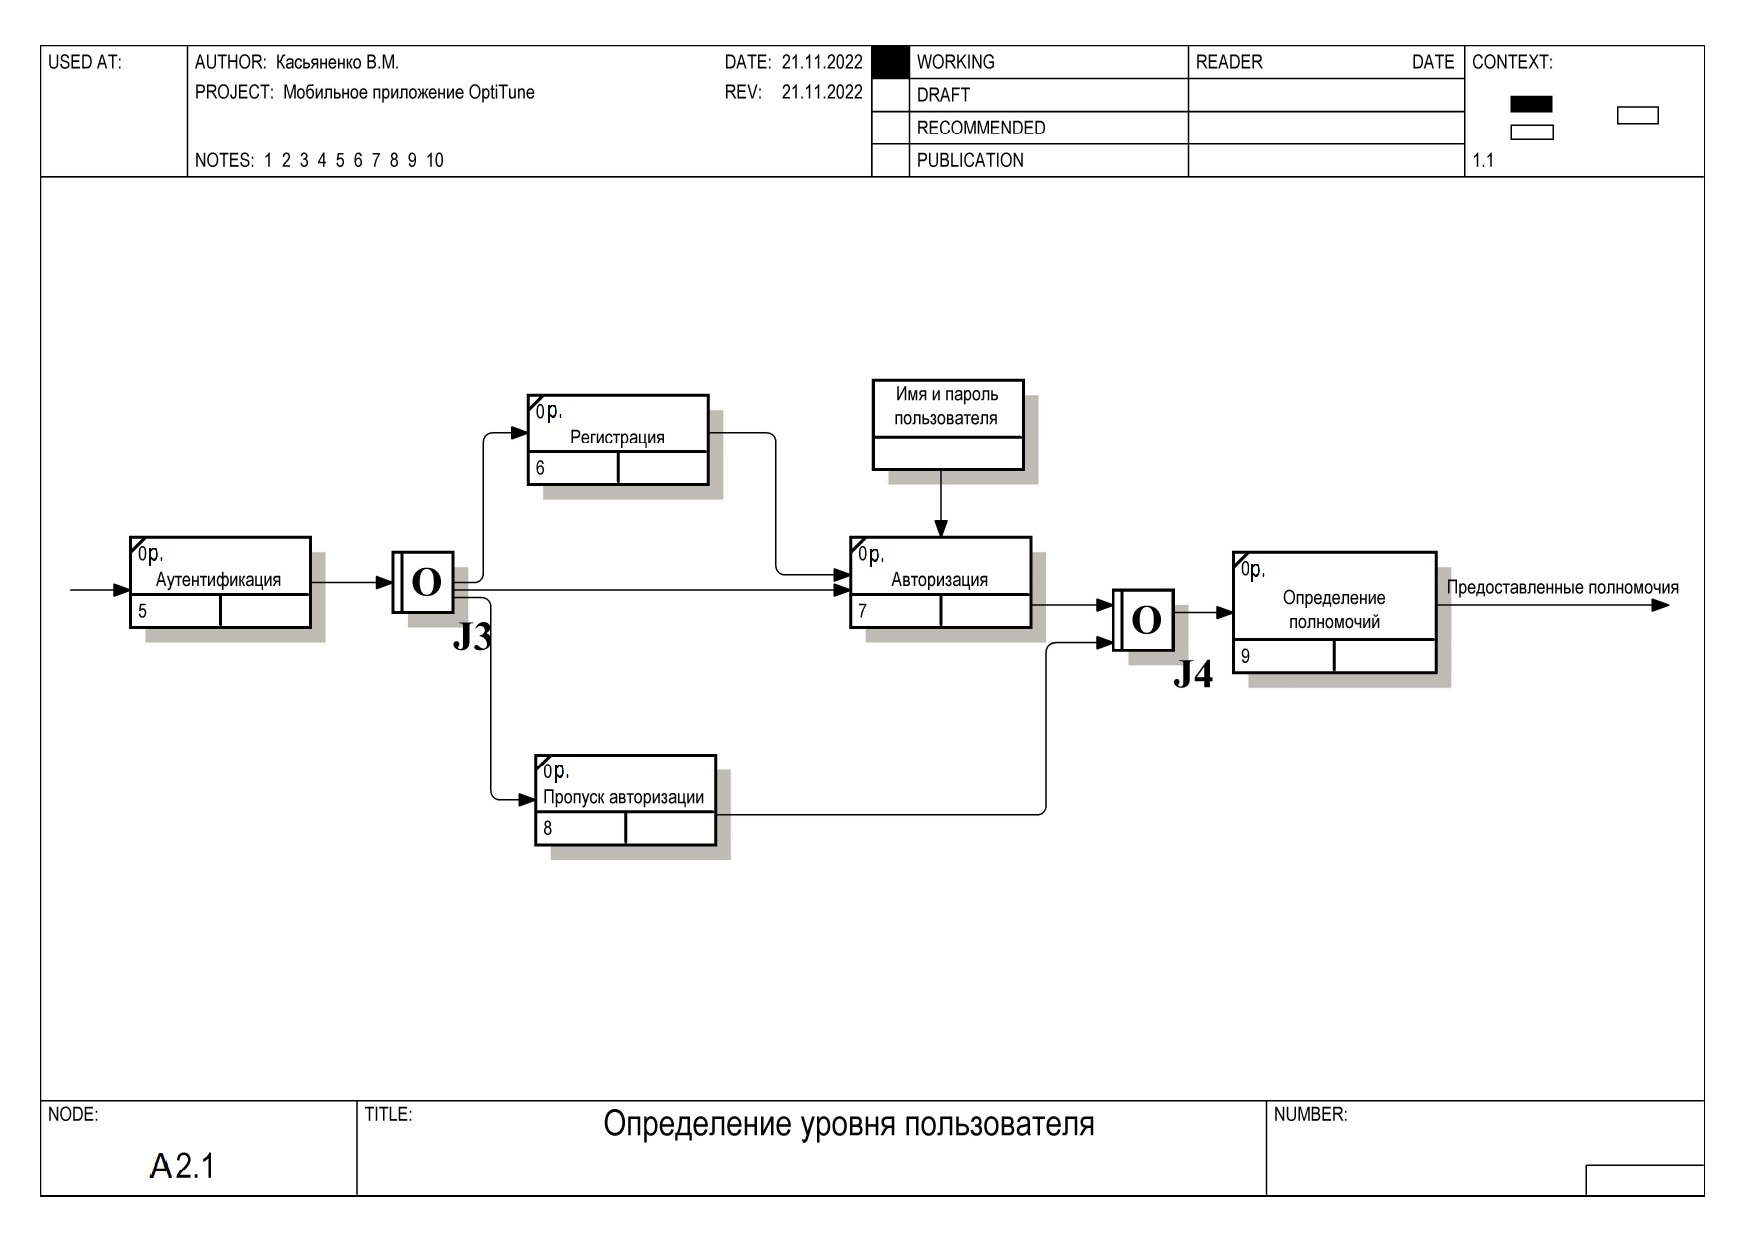
\includegraphics[width=0.9\linewidth]{idef312}}
\caption{Декомпозиция блока "Определение уровня доступа в систему"\ в стандарте IDEF3}
\label{fig20}
\end{figure}

\begin{figure}[H]
\centerline{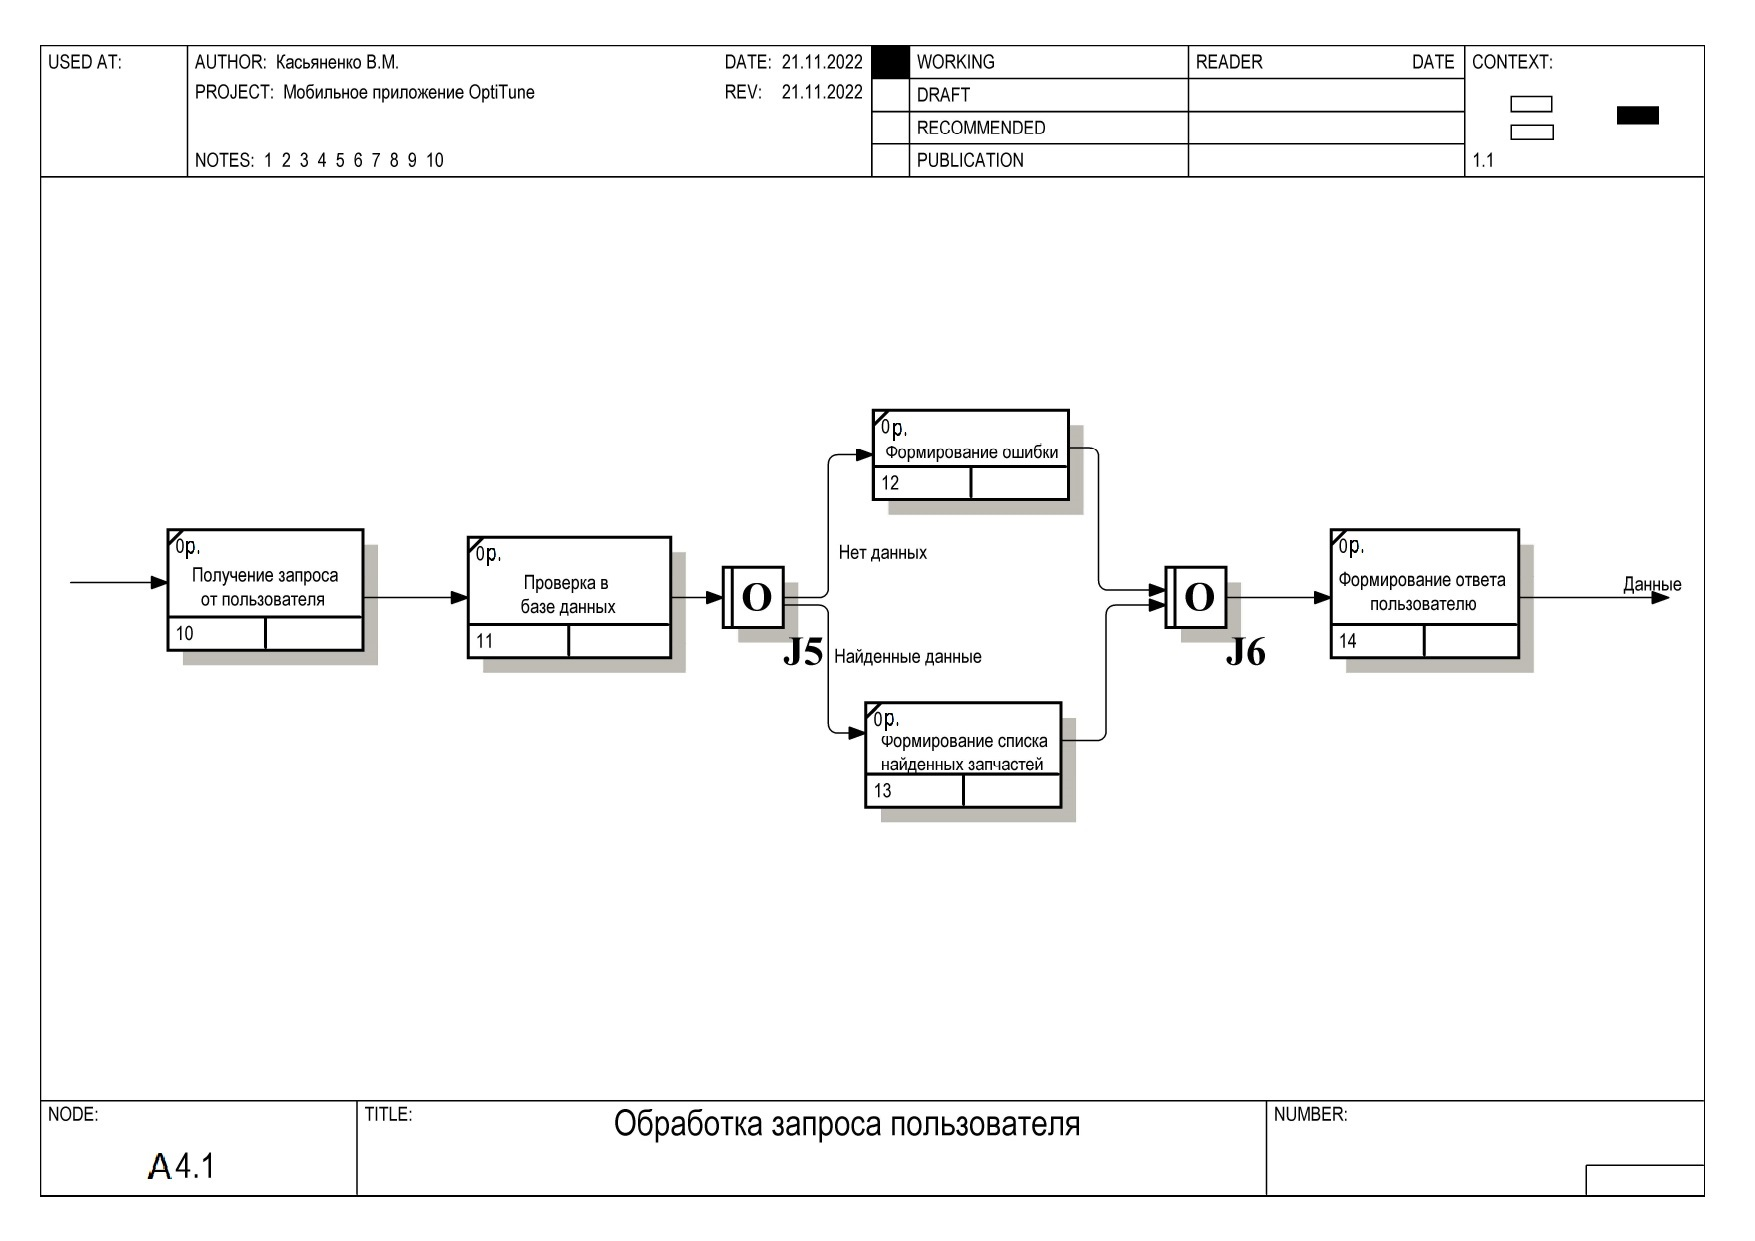
\includegraphics[width=0.9\linewidth]{idef313}}
\caption{Декомпозиция блока "Обработка запроса пользователя"\ в стандарте IDEF3}
\label{fig21}
\end{figure}
\end{landscape}





\chapter{Разработка технического задания на создание мобильного \\ приложения}

На основе предыдущей главы курсовой работы было разработано техническое задание на создание мобильного приложения OptiTune, выполненное в соответствии со стандартом качества \cite{bib7} и приведенное в данной главе.

\newpage
\section{Общие сведения}
\subsection{Наименование системы}
Наименование программного обеспечения: Мобильное приложение OptiTune.

\subsection{Плановые сроки начала и окончания работы по \\ созданию системы}
60 календарных дней с даты заключения контракта с Заказчиком.

\newpage
\section{Назначение и цели создания системы}
\subsection{Назначение системы}
Мобильное приложение OptiTune предназначено для использования профессиональными стрелками, охотниками и военными, позволяющее подобрать тюнинг для гладкоствольного и нарезного оружия, улучшив там самым качество стрельбы.

\subsection{Цели создания системы}

\begin{itemize}
	\item Ускорение поиска необходимого тюнинга для оружия;	
	\item Помощь в нахождении необходимого тюнинга.
\end{itemize}

\newpage
\section{Характеристика объектов автоматизации}

Объектом автоматизации является процесс поиска необходимого тюнинга в базе данных запчастей с использованием мобильных устройств.

Под мобильными устройствами в целях настоящего документа понимаются смартфоны и планшетные компьютеры, работающие под управлением мобильных операционных систем (iOS, Android) и имеющие доступ к сети Интернет.

\newpage
\section{Требования к приложению}
\subsection{Требования к системе в целом}
\subsubsection{Требования к режимам функционирования}
Для системы устанавливаются следующие режимы функционирования:
\begin{itemize}
	\item штатный режим функционирования;
	\item аварийный режим функционирования;
	\item сервисный режим функционирования.
\end{itemize}

Штатный режим является основным режимом функционирования приложения. В этом режиме должна быть обеспечена возможность доступа пользователей 
к приложению.

Система переходит в аварийный режим при возникновении нештатной ситуации и невозможности штатной работы. В случае перехода системы в аварийный режим, обслуживающему персоналу необходимо перевести систему в сервисный режим 
в соответствии с инструкциями, которые должны быть изложены в эксплуатационной документации.

Функционирование приложения при отказах и сбоях серверного оборудования не предусматривается.

В сервисном режиме система должна обеспечивать возможность проведения следующих работ:
\begin{itemize}
	\item техническое обслуживание;
	\item модернизацию аппаратно-программного комплекса;
	\item устранение аварийных ситуаций.
\end{itemize}

\subsubsection{Требования к численности и квалификации \\ персонала}
Минимальное количество персонала, требуемого для работы программы, должно
составлять не менее 3 штатных единиц — менеджер, модератор и консультант. Весь персонал должен иметь хорошие знания в области оружия и разбираться в нем.

Менеджер должен отвечать за базу данных запчастей, которую он обязан редактировать в случае обновления или появления новой информации.  В обязанности модератора входит проверка и публикация комментариев пользователей, а консультант должен отвечать на вопросы, которые отправляют ему авторизованные пользователи.

\subsubsection{Требования к надежности}
Спроектированные архитектурные решения системы должны быть устойчивы по отношению к программно-аппаратным ошибкам, отказам технических и программных средств, с возможностью восстановления ее работоспособности и целостности информационного содержимого при возникновении ошибок и отказов.

Некорректные действия пользователей не должны приводить к возникновению аварийной ситуации.

\subsubsection{Требования к эргономике и технической эстетике}
\begin{itemize}
	\item Взаимодействие пользователей с приложением должно осуществляться посредством визуального графического интерфейса;
	\item Интерфейс должен быть полностью русифицирован;
	\item Интерфейс не должен быть перегружен графическими элементами и должен обеспечивать быстрое отображение экранных форм;
	\item Пользователь должен иметь возможность указания критериев поиска и выбора информации без привлечения языков программирования;
	\item Элементы интерфейса (кнопки, ссылки) должны иметь названия, позволяющие пользователю однозначно интерпретировать выполняемые 
ими действия.
\end{itemize}

\subsubsection{Требования к защите информации от \\ несанкционированного доступа}
Система должна обеспечивать защиту авторизованных пользователей от несанкционированного доступа посредством следующих механизмов:
\begin{itemize}
	\item идентификация пользователя;
	\item проверка полномочий пользователя при работе с приложением;
	\item при наборе пароля его символы не показываются на экране, а заменяются одним типом символов.
\end{itemize}

\subsection{Требования к функциям, выполняемым системой}
Программа должна обеспечивать возможность выполнения перечисленных ниже
функций.

\subsubsection{Авторизация пользователя}
В приложении должна быть реализована авторизация пользователей. Пользователь может использовать приложение без авторизации, однако он получит доступ к полному функционалу только после завершения регистрации и последующей авторизации.

Процесс регистрации новых пользователей:
\begin{itemize}
	\item при запуске приложения пользователь может пройти регистрацию;
	\item регистрация проводится по логину, который придумает пользователь;
	\item программное обеспечение должно осуществлять поиск и проверку
введенного логина в базе данных пользователей;
	\item после успешной проверки пользователь вводит пароль
\end{itemize}

В случае успешной авторизации зарегистрированный пользователь получает доступ к полному функционалу приложения.

\subsubsection{Просмотр каталога}
В приложении должна быть реализована функция просмотра всего доступного тюнинга в виде ленты, которую можно пролистывать, а также при нажатии на иконку с какой-либо запчастью должно открываться окно просмотра этой запчасти В этом окне можно посмотреть данную запчасть в виде фотографий и 3D-моделей, которые можно масштабировать, а также рассматривать с разных ракурсов отдельно и на 3D-модели оружия, выбранного пользователем. Это позволит пользователю оценить насколько внешне подходит данная комплектация.

Также в окне просмотра запчасти должна быть доступна к просмотру и сравнению подробная характеристика этой запчасти, в которую входят такие параметры как вес, средняя цена на рынке, высота, ширина, толщина, материал, из которого изготовлена данная запчасть, а также остальные характеристики, доступные для той или иной запчасти. По этим характеристикам должна быть реализована функция сортировки в каталоге, что позволит пользователю быстрее найти необходимую запчасть.

В разделе просмотра каталога также должна быть реализована функция поиска по названию запчасти, в случае, если в базе запчастей не было найдено совпадений, должна выводиться ошибка пользователю. 

Более того, должна быть реализована функция добавления запчасти пользователем в избранное, а также удаление ее оттуда в разделах с каталогом, просмотром отдельных запчастей, а также в специальном разделе, где пользователь может посмотреть все запчасти, которые он добавил в избранное.

Пример дизайна интерфейса раздела "Каталог" представлен на рисунке \ref{fig22}. Выполнено с помощью \cite{bib8}.

\begin{figure}[H]
\centerline{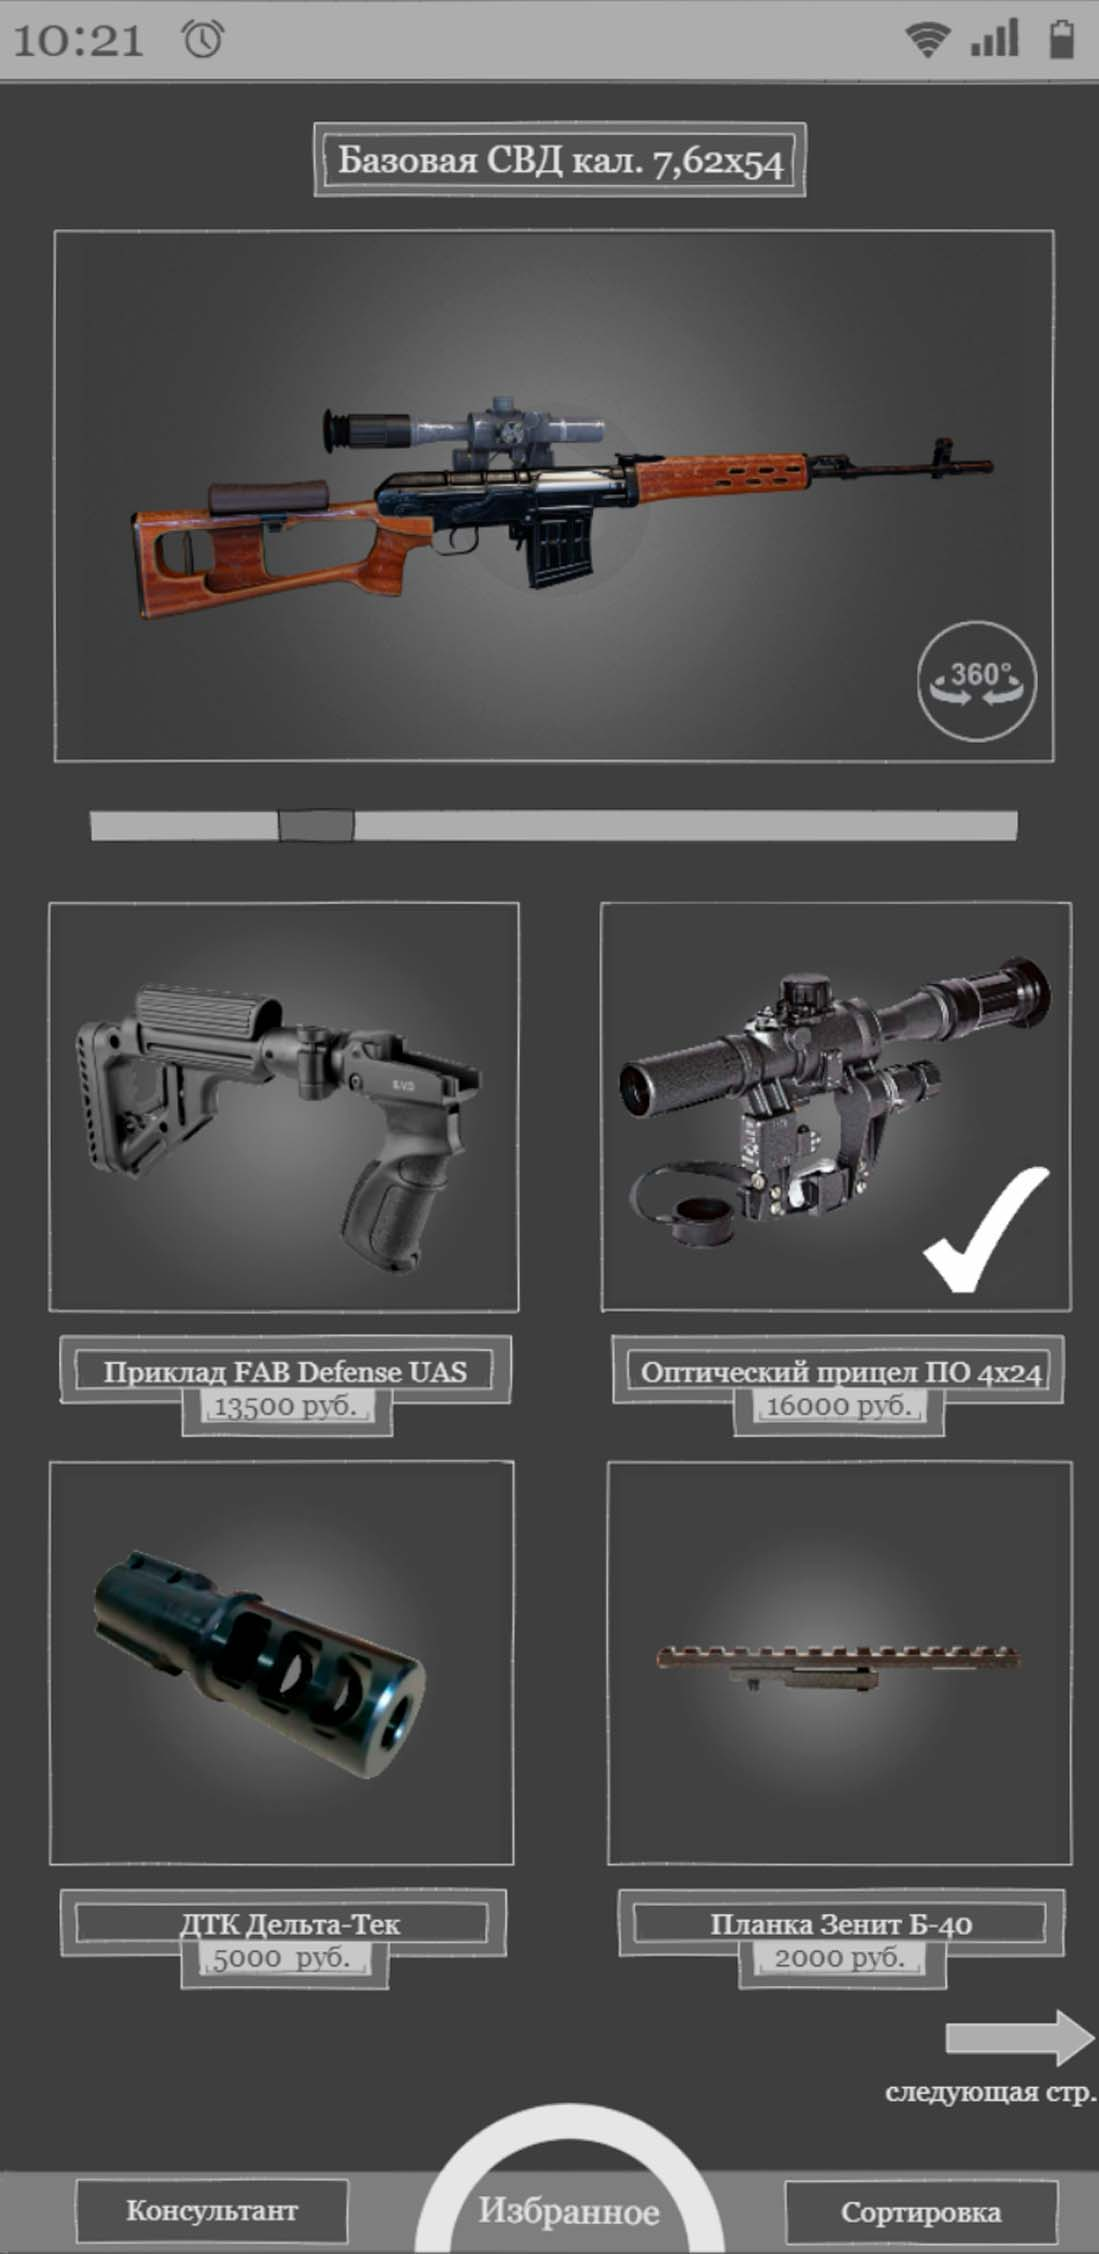
\includegraphics[width=0.6\linewidth]{pic}}
\caption{Пример дизайна интерфейса раздела "Каталог"}
\label{fig22}
\end{figure}

\subsubsection{Просмотр и написание комментариев}
В разделе просмотра отдельных запчастей должна быть реализована функция просмотра и написания комментариев с прикреплением приложений в виде фотографий и видеозаписей. Просмотр комментариев должен быть доступен всем пользователям приложения, а функция написания комментариев только авторизованным пользователям.

Процесс публикации комментариев:
\begin{itemize}
	\item написание комментария пользователем;
	\item отправка комментария на проверку модератором;
	\item публикация комментария модератором после успешной проверки. 
\end{itemize}

\subsubsection{Помощь онлайн-консультанта}
В приложении должна быть реализована функция помощи онлайн-консультанта для авторизованных пользователей. Необходимо обеспечить связь между пользователем и консультантом в отдельном разделе, где пользователь может написать вопрос по интересующей его запчасти или попросить рекомендацию у консультанта, который так же может написать ответное сообщение. 
 
\subsubsection{Настройки профиля}
Должна быть реализована функция настройки профиля в отдельном разделе, где авторизованный пользователь может изменить свой логин и пароль. Логин так же как и при регистрации проходит проверку на доступность.


\subsection{Требования к видам обеспечения}

\subsubsection{Требования к информационному обеспечению}
Проектирование структуры баз данных системы должно осуществляться с использованием инструмента проектирования на основе реляционного подхода.

Система должна быть организована рациональным способом, исключающим избыточную обработку, хранение и передачу информации.

\subsubsection{Требования к программному обеспечению}
Сервер системы управления базами данных должен функционировать под управлением операционной системы семейства MS Windows или аналогичной операционной системы. В качестве системы управления базами данных  используется Microsoft SQL Server версии 2008 и выше или PostgreSQL версии 9.3.X и выше, либо аналогичная реляционная система управления базами данных, обеспечивающая все функциональные возможности одного из перечисленных продуктов.

На мобильном устройстве пользователя должна быть установлена мобильная операционная система iOS версии 9 и выше или Android версии 4.4 и выше, а также приложение. 

\subsubsection{Требования к техническому обеспечению}
Техническое обеспечение системы должно максимально и наиболее эффективным образом использовать существующие у Заказчика технические средства.

Должно быть выделено серверное оборудования для сервера баз данных.

\subsubsection{Требования к организационному обеспечению}
Организационное обеспечение системы должно быть достаточным для эффективного выполнения персоналом возложенных на него обязанностей при осуществлении автоматизированных и связанных с ними неавтоматизированных функций приложения.

К работе с системой должны допускаться сотрудники, имеющие навыки работы за персональным компьютером, ознакомленные с правилами эксплуатации и прошедшие обучение работе с системой.

\newpage
\section{Состав и содержание работ по созданию приложения}
Разработка должна быть проведена в две стадии:
\begin{enumerate}
	\item Разработка приложения:
	\begin{itemize}
		\item проработка структуры приложения;
		\item разработка интерфейса;
		\item добавление запчастей, их характеристик и моделей в базу данных запчастей;
		\item создание функций сортировки и сравнения запчастей по их характеристикам;
		\item разработка системы аутентификации пользователей;
		\item создание функции добавления запчастей в избранное;
		\item создание функции комментирования;
		\item создание функции обращения к онлайн-консультанту;
		\item тестирование, а также устранение выявленных ошибок в работе приложения;
	\end{itemize}
	\item Загрузка приложений в общий доступ:
	\begin{itemize}
		\item загрузка приложения в App Store;
		\item загрузка приложения в Google Play.
	\end{itemize}
\end{enumerate} 

\newpage
\section{Порядок контроля и приемки приложения}

Тестирование системы должно проводиться по следующим этапам:
\begin{itemize}
	\item тестирование регистрации пользователя;
	\item тестирование авторизации пользователя;
	\item тестирование изменений логина и пароля пользователя;
	\item тестирование функции изменения базы данных запчастей;
	\item тестирование основных функций приложения - просмотр и поиск в каталоге, просмотр запчастей в 3D-виде, добавление и удаление запчастей из избранного, сравнение запчастей по характеристикам;
	\item тестирование ситуации "не нашлось совпадений по запросу"\ в каталоге;
	\item тестирование работы кнопок перехода между вкладками;
	\item тестирование функций просмотра и добавления комментариев;
	\item тестирование общения пользователя с онлайн-консультантом через специальное окно.
\end{itemize}

Ответственность за организацию и проведение приемки системы должен нести Заказчик. Приемка системы должна производиться по завершению приемки всех задач системы. При этом необходимо предоставить обеспечение материальной частью (технические средства), проектной документацией и специально выделенным персоналом.

Заказчик должен предъявлять систему ведомственной приемочной комиссии, при этом он обязан обеспечить нормальные условия работы данной комиссии в соответствии с принятой программой приемки.

Завершающим этапом при приемке системы должно быть составление акта приемки.

\newpage
\section{Требования к составу и содержанию работ по подготовке \\
объекта автоматизации к вводу системы в действие}
Для обеспечения готовности объекта к вводу системы в действие провести комплекс мероприятий:
\begin{itemize}
	\item приобрести компоненты технического и программного обеспечения, заключить договоры на их лицензионное использование;
	\item завершить работы по установке технических средств;
	\item провести обучение членов административной группы
\end{itemize}

\newpage
\section{Требования к документированию}
Документация должна разрабатываться с учетом требований комплекса государственных стандартов «Информационная технология. Комплекс стандартов на автоматизированные системы»:
\begin{itemize}
	\item ГОСТ 34.601–90 «Автоматизированные системы. Стадии создания»;
	\item ГОСТ 34.003–90 «Автоматизированные системы. Термины и определения»;
	\item ГОСТ 34.602–89 «Техническое задание на создание автоматизированной системы»;
	\item ГОСТ 34.201–89 «Виды, комплектность и обозначение документов при создании автоматизированных систем»;
	\item ГОСТ 34.603–92 «Виды испытаний автоматизированных систем».
\end{itemize}

Документация должна включать следующие документы:
\begin{itemize}
	\item Техническое задание на разработку мобильного приложения;
	\item Программа и методика испытаний приложения;
	\item Руководство менеджера приложения;
	\item Руководство модератора приложения;
	\item Руководство ассистента приложения;
	\item Руководство пользователя приложения.
\end{itemize}

Вся документация должна быть выполнена на русском языке и передана заказчику в печатном виде в одном экземпляре, а также в электронном виде в одном экземпляре в формате doc, docx или pdf.

\newpage
\section{Источники разработки}
Документ, на основе которого разрабатывалось техническое задание и которое должно быть использовано при создании системы:
\begin{itemize}
	\item ГОСТ 34.602-89. Информационная технология. Комплекс стандартов на автоматизированные системы. Техническое задание на создание автоматизированной системы.
\end{itemize}


\conclusions

В процессе написания курсовой работы были решены следующие задачи:
\begin{itemize}
	\item описаны основные функции приложения, а также его пользователи;
	\item проведен обзор аналогов;
	\item обоснована необходимость создания данного приложения;
	\item разработаны диаграммы прецедентов и активности для типовых сценариев работы приложения;
	\item разработаны диаграммы IDEF0, DFD, IDEF3 для будущего приложения.
\end{itemize}

Более того, была решена основная задача, а также достигнута цель курсовой работы: разработка технического задания на создание мобильного приложения OptiTune. Представленное техническое задание будет использовано при дальнейшей реализации и разработке приложения. 

Также необходимо отметить, что при написании курсовой работы был получен опыт создания моделей и диаграмм в различных стандартах, а также был получен опыт создания технического задания, что поможет при дальнейшей реализации и развитии мобильного приложения OptiTune.


\newpage
\begin{thebibliography}{99}

\bibitem{bib1} Custom Guns: официальный сайт. – URL: \url{https://custom-guns.ru} (Дата обращения 11.10.2022).

\bibitem{bib2} QUARTA: официальный сайт. – URL: \url{https://quarta-hunt.ru} (Дата обращения 11.10.2022).

\bibitem{bib3} Guns parts: официальный сайт. – URL: \url{https://www.gunsparts.ru} (Дата обращения 11.10.2022).

\bibitem{bib4} StarUML: официальный сайт. – URL: \url{https://staruml.io/} (Дата обращения 29.10.2022).

\bibitem{bib5} Ramus: официальный сайт. – URL: \url{https://ramussoftware.com/} (Дата обращения 25.11.2022).

\bibitem{bib6} ERwin: официальный сайт. – URL: \url{https://www.erwin.com/} (Дата обращения 25.11.2022).

\bibitem{bib7} ГОСТ 34.602-89. Информационная технология. Комплекс стандартов на автоматизированные системы. Техническое задание на создание автоматизированной системы.

\bibitem{bib8} NinjaMock: официальный сайт. – URL: \url{https://ninjamock.com/} (Дата обращения 12.10.2022).

\end{thebibliography}

\end{document}